\documentclass{standalone}
\usepackage{tikz}
\begin{document}
	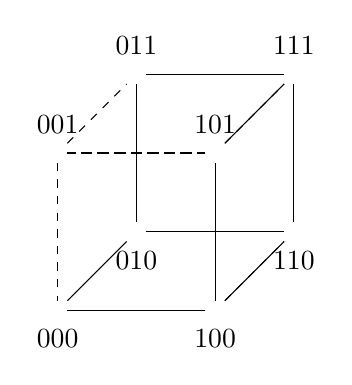
\begin{tikzpicture} 
	\pgfsetxvec{\pgfpoint{1.cm}{0.0cm}} 
	\pgfsetyvec{\pgfpoint{0.0cm}{1.0cm}} 

	\node[] at (2.5,1.5) [label=below:$000$] (000) {}; 
	\node[] at (4.5,1.5) [label=below:$100$] (100) {}; 
	\node[] at (2.5,3.5) [label=above:$001$] (001) {}; 
	\node[] at (4.5,3.5) [label=above:$101$] (101) {}; 
	\node[] at (3.5,2.5) [label=below:$010$] (010) {}; 
	\node[] at (5.5,2.5) [label=below:$110$] (110) {}; 
	\node[] at (3.5,4.5) [label=above:$011$] (011) {}; 
	\node[] at (5.5,4.5) [label=above:$111$] (111) {}; 
	\path (010) 
	edge (110) 
	edge (011) 
	edge (000) 
	(100)	
	edge (000) 
	edge (110) 
	edge (101) 
	(111)	
	edge (110) 
	edge (101) 
	edge (011); 
	\path[dashed](101) 
	edge (001)	
	edge (100) 
	edge (111) 
	(100) 
	edge (110)	
	edge (000) 
	edge (101)
	(001)
	edge (011)
	edge (000)
	edge (101); 

	\end{tikzpicture} 
\end{document}